% =============================================================
%  Asking for Properties: A Conditional Transformer VAE
%  Series B: Deep Learning for Molecules, Post 6b
%  Compiles with pdfLaTeX on Overleaf (no extra files needed).
% =============================================================
\documentclass[11pt]{article}

\usepackage[margin=1in]{geometry}
\usepackage[T1]{fontenc}
\usepackage{lmodern}
\usepackage{microtype}
\usepackage{amsmath,amssymb,bm}
\usepackage{booktabs}
\usepackage{enumitem}
\usepackage{xcolor}
\usepackage{listings}
\usepackage{tikz}
\usetikzlibrary{arrows.meta,positioning,calc}
\usepackage{pgfplots}
\pgfplotsset{compat=1.16}
\usepackage[most]{tcolorbox}
\usepackage[colorlinks=true,linkcolor=blue!50!black,urlcolor=blue!50!black]{hyperref}

\setlength{\parskip}{0.55em}
\setlength{\parindent}{0pt}

% ---------- macros ----------
\newcommand{\T}{\mathsf{T}}
\newcommand{\E}{\mathbb{E}}
\newcommand{\R}{\mathbb{R}}
\DeclareMathOperator{\Var}{Var}
\DeclareMathOperator{\MMD}{MMD}

% ---------- Colab links: edit these lines after you upload the notebooks to GitHub ----------
\newcommand{\colaburlfull}{https://colab.research.google.com/github/YOUR-USER/YOUR-REPO/blob/main/notebooks/TCVAE_Tutorial.ipynb}
\newcommand{\colaburlprimer}{https://colab.research.google.com/github/YOUR-USER/YOUR-REPO/blob/main/notebooks/B6b_cvae_primer_colab.ipynb}
\newcommand{\colabbutton}[2]{%
  \href{#1}{\tcbox[on line,colback=orange!15,colframe=orange!70!black,boxrule=0.6pt,arc=3pt,
    left=4pt,right=4pt,top=1pt,bottom=1pt]{\small\textbf{$\blacktriangleright$ #2}}}}
\newcommand{\tryit}[1]{\par\vspace{0.3em}\noindent
  \fcolorbox{orange!70!black}{orange!8}{\parbox{\dimexpr\linewidth-2\fboxsep-2\fboxrule\relax}{%
  \small $\blacktriangleright$ \textbf{Run it.} #1}}\par\vspace{0.3em}}

% ---------- code listings ----------
\definecolor{codebg}{RGB}{246,246,248}
\definecolor{codecomment}{RGB}{90,110,90}
\definecolor{codekw}{RGB}{30,60,160}
\lstset{
  language=Python,
  basicstyle=\ttfamily\small,
  keywordstyle=\color{codekw}\bfseries,
  commentstyle=\color{codecomment}\itshape,
  backgroundcolor=\color{codebg},
  frame=single,
  rulecolor=\color{black!15},
  breaklines=true,
  columns=fullflexible,
  showstringspaces=false,
  xleftmargin=0.5em,
  xrightmargin=0.5em,
  aboveskip=0.8em,
  belowskip=0.8em
}

% ---------- boxes ----------
\tcbuselibrary{skins,breakable}
\newtcolorbox{keybox}[1][]{
  enhanced, breakable, colback=blue!4, colframe=blue!50!black,
  fonttitle=\bfseries, title={#1}, boxrule=0.6pt, arc=2pt
}
\newtcolorbox{mathbox}[1][]{
  enhanced, breakable, colback=black!3, colframe=black!45,
  fonttitle=\bfseries, title={#1}, boxrule=0.6pt, arc=2pt
}
\newtcolorbox{warnbox}[1][]{
  enhanced, breakable, colback=red!4, colframe=red!60!black,
  fonttitle=\bfseries, title={#1}, boxrule=0.6pt, arc=2pt
}
\newtcolorbox{hypbox}[1][]{
  enhanced, breakable, colback=yellow!8, colframe=yellow!50!black,
  fonttitle=\bfseries, title={#1}, boxrule=0.6pt, arc=2pt
}

% ---------- title ----------
\title{\textbf{Asking for Properties:}\\[0.2em]
       A Conditional Transformer VAE}
\author{\textit{Series B: Deep Learning for Molecules --- Post 6b}}
\date{}

\begin{document}
\maketitle
\thispagestyle{empty}

\begin{center}
\small
About 35 minutes of reading, plus the notebooks.\\
\textbf{Prerequisites:} Post B6 (the unconditional VAE Transformer) and Post A2 (neural networks).\\[0.5em]
\textbf{Notebook 1, the full tutorial:} \texttt{TCVAE\_Tutorial.ipynb} (GPU runtime, pre-trained model)\\
\textbf{Notebook 2, the primer:} \texttt{B6b\_cvae\_primer\_colab.ipynb} (CPU only, no model file)\\[0.4em]
\colabbutton{\colaburlfull}{Open the full tutorial}\quad
\colabbutton{\colaburlprimer}{Open the primer}\quad
{\footnotesize (see Section~\ref{sec:runit})}
\end{center}

\vspace{0.5em}
\hrule
\vspace{0.5em}

% =============================================================
\section{The question}
% =============================================================
In drug discovery we rarely want \emph{any} new molecule. We want molecules with specific properties: a certain solubility, a high drug-likeness, an easy synthesis. The model of Post~B6 gave us no handle on these. A standard VAE describes the distribution of molecules $p(x)$, so sampling from it returns molecules with whatever properties the training set happened to have.

A \textbf{conditional} model describes the distribution of molecules \emph{given} a set of properties $c$, written $p(x\mid c)$. Fix $c$, sample at random, and we should get many different molecules that all have properties close to $c$. This post builds such a model, a \textbf{conditional VAE with a Transformer} (TCVAE), by adding three numbers to the input.

The more important part is the \emph{testing}. A model that accepts a request has not necessarily honored it. We will measure the requested properties of the generated molecules with an independent calculation, and ask three questions: does the model use the condition at all, how closely does it follow it, and where does it break? The answers are more nuanced than ``it works,'' and one of them traces back to a detail of the latent space that Post~B6 set up.

\begin{keybox}[Where the numbers come from]
The model is the pre-trained TCVAE in the tutorial notebook of Prof.\ V.~S.~Batista's CHEM~584 course (an earlier version was designed by Dr.\ H.~Li). The data facts of Step~1, the parameter count, and all of the mathematics are recomputed in the primer notebook. Numbers that describe the \emph{trained model} (probe $R^2$, sampling metrics, the property scans) are taken from the saved output of one run of the tutorial notebook on a T4 GPU, seed~0; quantities read off a figure are marked ``approximately.'' Running the notebook yourself should give numbers within the quoted error bars, not necessarily identical ones.
\end{keybox}

% =============================================================
\section{Step 1: From properties to condition tokens}
% =============================================================
The model reads discrete tokens, so each continuous property must be \textbf{discretized}. For each of three properties (LogP, the octanol--water partition coefficient; QED, a drug-likeness score between 0 and 1; and SAS, the synthetic-accessibility score) we cut the range between its smallest and largest value in the data into \textbf{50 equal-width classes}, numbered 0 to 49. Each class then becomes a token, like a SMILES character:

\begin{center}
\small
\begin{tabular}{@{}lccc@{}}
\toprule
Property & Range in the data & Class width & Token numbers\\
\midrule
LogP & $[-6.876,\ 8.252]$ & $0.303$ & $40$ to $89$\\
QED & $[0.112,\ 0.948]$ & $0.0167$ & $90$ to $139$\\
SAS & $[1.133,\ 7.289]$ & $0.123$ & $140$ to $189$\\
\bottomrule
\end{tabular}
\end{center}

The SMILES characters and the padding token use $0$ to $36$, so the condition tokens start at $40$ (the numbers $37$ to $39$ stay unused). Three condition tokens are appended to every row, after the padded SMILES tokens, so each row has $112+3=115$ entries. For example, the first molecule of the data set has tokens $[79,125,147]$, which means LogP class $39$, QED class $35$ and SAS class $7$, that is, LogP in $[4.92,5.23]$, QED in $[0.70,0.71]$ and SAS in $[1.99,2.12]$. Because the order is fixed, the model always knows which property a condition token refers to.

\subsection*{How well populated are the classes?}
Equal-width classes are simple, but the property distributions are far from flat. For LogP, counting all $249{,}455$ molecules of the data set:

\begin{center}
\small
\begin{tabular}{@{}lccccccccc@{}}
\toprule
LogP class & 5 & 10 & 15 & 20 & 25 & 30 & 35 & 40 & 45\\
Molecules in class & 4 & 37 & 406 & 2380 & 9368 & 20044 & 16067 & 1328 & 7\\
\bottomrule
\end{tabular}
\end{center}

The classes at the edges of the range are almost empty. The situation is sharper still for the \emph{combination} of the three properties. There are $50^3=125{,}000$ possible (LogP, QED, SAS) cells, of which $22{,}148$ are occupied, with a median of 4 molecules per occupied cell. The notebook's ``typical'' request, classes $(39,35,7)$, matches exactly $4$ molecules. The model cannot work by looking up the contents of a cell; it has to generalize across neighboring classes.

The properties are also correlated: $-0.52$ between LogP and SAS, $-0.17$ between LogP and QED, $+0.10$ between QED and SAS. A request for a very water-soluble molecule (low LogP) with arbitrary QED and SAS may ask for a combination that hardly exists. We will test this.

\subsection*{Are the file's labels the ones we will measure?}
Later we measure generated molecules with RDKit, so ``requested'' and ``measured'' must be on the same scale. The notebook recomputes the properties of $1000$ random molecules with RDKit and compares them with the stored values. The LogP values agree to rounding (mean absolute difference $0.000$), and the QED values agree to $0.013$ on average, small but not zero, with a visible scatter. (SAS needs an extra RDKit module and is not rechecked.) So part of any later disagreement in QED could come from the labels and not from the model.

\tryit{Primer \S1. Recompute the class edges from the data file, reproduce the tokens $[79,125,147]$, the class counts above, the $22{,}148$ occupied cells, and the correlations.}

% =============================================================
\section{Step 2: What the condition changes in the model}
% =============================================================
The model is the Transformer autoencoder of Post~B6 (6 encoder and 6 decoder layers, 4 heads, embedding size 128, a latent vector $\bm z$ of $10\times128=1280$ numbers, noise of standard deviation 1 added to $\bm z$ during training). Two small changes make it conditional (Figure~\ref{fig:arch}):

\begin{enumerate}[nosep]
  \item \textbf{The encoder also returns the embeddings of the three condition tokens.} The condition tokens are part of the input row, so the encoder's attention layers see them. In addition, the encoder returns their \emph{raw} token embeddings, taken straight from the embedding table before positional information and attention: a $3\times128$ array $\bm c$, flattened to $384$ numbers.
  \item \textbf{The decoder input is $[\bm z\,|\,\bm c]$.} The noised latent vector is concatenated with $\bm c$, giving $1280+384=1664$ numbers, which one linear layer maps to the $10\times128$ ``memory'' that the decoder attends to.
\end{enumerate}

\begin{figure}[ht]
\centering
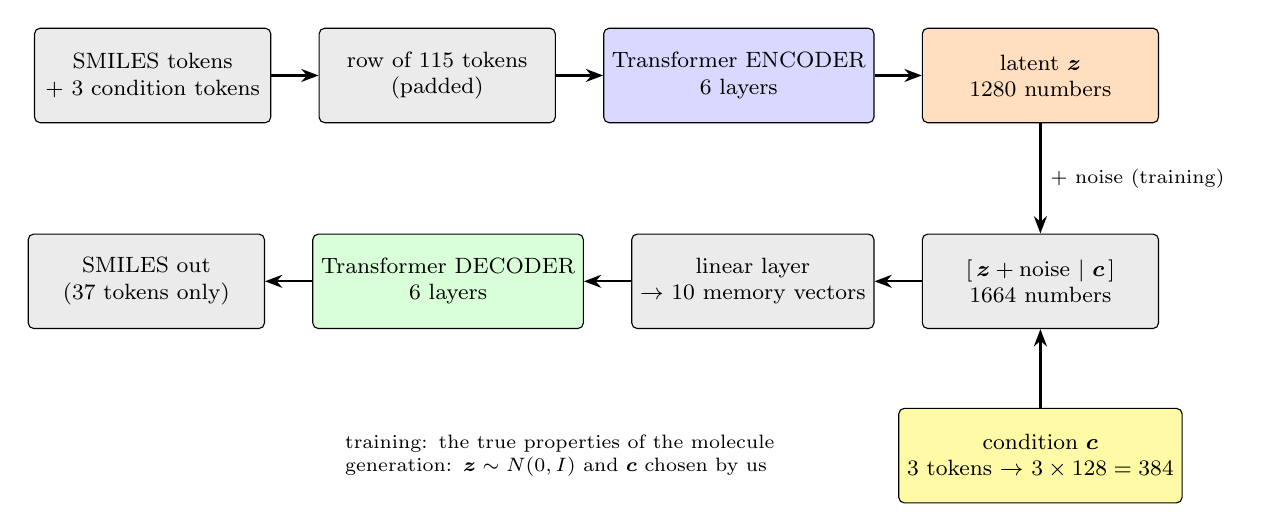
\begin{tikzpicture}[
  box/.style={draw, rounded corners=2pt, minimum height=1.2cm, minimum width=3.0cm, align=center, font=\footnotesize, inner sep=3pt},
  gray/.style={box, fill=black!8},
  enc/.style={box, fill=blue!15},
  dec/.style={box, fill=green!15},
  lat/.style={box, fill=orange!25},
  cond/.style={box, fill=yellow!35},
  arr/.style={-{Stealth[length=2.2mm]}, thick}
]
% row 1: encoding
\node[gray] (smi) {SMILES tokens\\+ 3 condition tokens};
\node[gray, right=0.6cm of smi] (tok) {row of 115 tokens\\(padded)};
\node[enc, right=0.6cm of tok] (enc) {Transformer ENCODER\\6 layers};
\node[lat, right=0.6cm of enc] (z) {latent $\bm z$\\1280 numbers};
\draw[arr] (smi) -- (tok); \draw[arr] (tok) -- (enc); \draw[arr] (enc) -- (z);
% row 2: decoding (right to left)
\node[gray, below=1.4cm of z] (cat) {$[\,\bm z+\text{noise}\ |\ \bm c\,]$\\1664 numbers};
\node[gray, left=0.6cm of cat] (inv) {linear layer\\$\to$ 10 memory vectors};
\node[dec, left=0.6cm of inv] (dec) {Transformer DECODER\\6 layers};
\node[gray, left=0.6cm of dec] (out) {SMILES out\\(37 tokens only)};
\draw[arr] (z) -- node[right, font=\scriptsize]{$+$ noise (training)} (cat);
\draw[arr] (cat) -- (inv); \draw[arr] (inv) -- (dec); \draw[arr] (dec) -- (out);
% condition
\node[cond, below=1.0cm of cat] (c) {condition $\bm c$\\3 tokens $\to$ $3\times128=384$};
\draw[arr] (c) -- (cat);
\node[font=\scriptsize, text width=6.5cm, align=left, left=0.4cm of c] {training: the true properties of the molecule\\generation: $\bm z\sim N(0,I)$ and $\bm c$ chosen by us};
\end{tikzpicture}
\caption{The conditional model. The encoder compresses the row (SMILES plus condition tokens) into $\bm z$. The decoder receives $\bm z$ (with noise during training) concatenated with the clean condition embedding $\bm c$. To generate, we skip the encoder: $\bm z$ is drawn from $N(0,I)$ and $\bm c$ is the embedding of the condition we request. The decoder only ever writes the 37 SMILES tokens.}
\label{fig:arch}
\end{figure}

Three details of the design are worth noting. The noise is added to $\bm z$ only: the condition embedding $\bm c$ always arrives clean. The decoder's output vocabulary stays at $37$ tokens, so it cannot write condition tokens. And the two residual blocks of the unconditional model are gone.

Counting parameters shows what the condition added (\hyperref[sec:S3]{Supplement S3} derives each line; the total matches the $23{,}046{,}693$ printed by the tutorial):

\begin{center}
\small
\begin{tabular}{@{}lrr@{}}
\toprule
Component & Parameters & Share\\
\midrule
Encoder embeddings ($190$ tokens, $200$ positions) & $49{,}920$ & $0.2\%$\\
Encoder layers (6) & $794{,}880$ & $3.4\%$\\
Decoder embeddings ($37$ tokens, $200$ positions) & $30{,}336$ & $0.1\%$\\
Decoder layers (6) & $1{,}192{,}704$ & $5.2\%$\\
Decoder output layer & $4{,}773$ & $0.0\%$\\
\textbf{Latent layer} ($14{,}720\to1280$) & $18{,}842{,}880$ & $\mathbf{81.8\%}$\\
Inverse layer ($1664\to1280$) & $2{,}131{,}200$ & $9.2\%$\\
\midrule
Total & $23{,}046{,}693$ & $100\%$\\
\bottomrule
\end{tabular}
\end{center}

Compared with the $21{,}859{,}969$ parameters of Post~B6, the condition adds $1{,}186{,}724$, almost all of it from two layers getting wider: $+655{,}360$ in the latent layer (input $115\times128$ instead of $111\times128$) and $+491{,}520$ in the inverse layer ($1664$ instead of $1280$ inputs). The condition itself, as embeddings, costs very little; the cost is mostly in how the rest of the model reads it.

\tryit{Primer \S2. Derive the table and the change of $+1{,}186{,}724$ from the architecture.}

% =============================================================
\section{Step 3: Training, briefly}
% =============================================================
The objective is the same as in Post~B6: cross-entropy (rebuild the SMILES string, ignoring padding) plus the MMD penalty, with Adam, teacher forcing, and fresh prior samples at each step. Two differences are worth knowing. The penalty weight is $4$ instead of $8$, and, unlike the unconditional tutorial where the weight had to be increased gradually, this model is trained with a \emph{single} set of parameters. The notebook reports about 50 minutes of GPU time for $10$ epochs for results similar to the pre-trained model, and, as before, does not recommend retraining by default; the target for training is the SMILES tokens only, and the condition tokens are inputs.

% =============================================================
\section{Step 4: Two checks before we use the condition}
% =============================================================
\subsection*{4a. Does the latent space match its prior?}
Exactly the diagnostics of Post~B6, on $2000$ encoded test molecules:

\begin{center}
\begin{tabular}{@{}lcc@{}}
\toprule
 & Encoded molecules & Prior $N(0,I)$\\
\midrule
Mean vector length $\lVert\bm z\rVert$ & $11.8$ & $35.8$\\
Mean standard deviation of a coordinate & $0.33$ & $1$\\
Penalty value vs.\ the prior & $3.282$ & $3.820$ (prior vs.\ prior)\\
\bottomrule
\end{tabular}
\end{center}

The story is the same as before, only more pronounced: the encoded vectors are about three times shorter than prior draws. There is, however, a sharper way to say what the simplified penalty does. Because the prior samples are isotropic Gaussians, the average kernel value between a vector $\bm z$ and the prior depends on $\bm z$ \textbf{only through its length} (Supplement~\hyperref[sec:S4]{S4}):
\begin{equation}
  \text{penalty}=w\Big[1-\Big(1+\tfrac2s\Big)^{-d/2}\,\overline{\exp\!\Big(-\frac{\lVert\bm z\rVert^2}{s+2}\Big)}\Big],\qquad w=4,\ s=819.2,\ d=1280 .
  \label{eq:lenpen}
\end{equation}
This is minimal at $\lVert\bm z\rVert=0$ and increases with the length, and it cannot tell one direction from another. The numbers fit:

\begin{center}
\small
\begin{tabular}{@{}lcc@{}}
\toprule
Case & Penalty from Eq.~\eqref{eq:lenpen} & Measured\\
\midrule
Two prior samples (length $\approx35.8$) & $3.823$ & $3.820$\\
Encoded molecules ($\lVert\bm z\rVert=11.8$) & $3.291$ & $3.282$\\
All vectors at the origin & $3.160$ & ---\\
\bottomrule
\end{tabular}
\end{center}

(Applying the same formula to the unconditional model of Post~B6, with weight $8$ and $\lVert\bm z\rVert=14.3$, gives $6.690$ against the $6.672$ measured there.)

\begin{keybox}[A test that passes while the vectors are three times too short]
In the tutorial's Figure~6a, the histogram of the first principal component of the encoded vectors looks almost exactly like the null reference. Yet Figure~6c shows the vectors are about a third of the prior's length. The principal-component test is blind to length, because with $n=2000$ points in $1280$ dimensions even perfect Gaussian data has a first component of standard deviation $1+\sqrt{d/n}\approx1.8$ (and $3.2$ for a batch of $256$). Always look at the length distribution too.
\end{keybox}

As in Post~B6, sampling still works because of the noise added during training. The decoder's training input is $\bm z+\bm\varepsilon$ with per-coordinate spread $\sqrt{0.33^2+1}=1.05$, so its length is about $\sqrt{1280\cdot1.109}=37.7$, close to the $35.8$ of a prior draw.

\tryit{Primer \S3. Evaluate Eq.~\eqref{eq:lenpen}, then construct two sets of vectors with the same length but very different shapes (one with $88\%$ of its variance in 20 of 1280 coordinates) and watch their penalties agree.}

\subsection*{4b. Does the latent vector carry the properties?}
This question is specific to conditional models. If $\bm z$ already encodes LogP, QED or SAS, the decoder can read them from $\bm z$ and may pay less attention to $\bm c$, which weakens the control we want. The tutorial tests this with a ridge regression that predicts each property from $\bm z$ (fit on $1500$ test molecules, scored with $R^2$ on the other $500$), and repeats the fit with shuffled labels:

\begin{center}
\begin{tabular}{@{}lcc@{}}
\toprule
Property & $R^2$ from $\bm z$ (held out) & $R^2$, shuffled labels\\
\midrule
LogP & $0.617$ & $-0.013$\\
QED & $0.624$ & $-0.006$\\
SAS & $0.742$ & $-0.006$\\
\bottomrule
\end{tabular}
\end{center}

The latent vector carries a lot of \emph{linearly decodable} information about all three properties: $62$ to $74\%$ of the variance. (A linear probe is only a lower bound.) The condition is therefore not the only route by which the decoder can learn a molecule's properties. Keep this in mind for Step~6.

% =============================================================
\section{Step 5: Sampling with a typical condition}
% =============================================================
Now the first generation test. Draw $5000$ random latent vectors and decode them all with the \emph{typical} condition $(39,35,7)$, where the data are abundant. Metrics as in Post~B6:

\begin{center}
\small
\begin{tabular}{@{}lccc@{}}
\toprule
Metric & Count & Out of & Percent (95\% CI)\\
\midrule
Parses as SMILES (grammar only) & $4975$ & $5000$ & $99.50\pm0.20$\\
\textbf{Chemically valid} & $4882$ & $5000$ & $\mathbf{97.64}\pm0.42$\\
Repeated (among valid) & $21$ & $4882$ & $0.43\pm0.18$\\
Novel (among distinct valid) & $4857$ & $4861$ & $99.92\pm0.08$\\
Exactly reconstructed (test) & $2660$ & $5000$ & $53.20\pm1.38$\\
\bottomrule
\end{tabular}
\end{center}

The yield of new, distinct, valid molecules is validity $\times$ uniqueness $\times$ novelty $=0.9764\times0.9957\times0.9992=97.14\%$, or $4857$ of $5000$. The failures are few and of two kinds: $1.86\%$ Kekulization errors (an aromatic ring that cannot be written with alternating bonds) and $0.50\%$ syntax errors.

\textbf{Be careful about comparing with Post~B6.} There, $79.4\%$ of samples were valid and $68.6\%$ of test molecules were reconstructed exactly; here the figures are $97.6\%$ and $53.2\%$. The notebook itself notes that the two models were trained differently, and there is a second difference: this test uses \emph{one} dense, typical request. Step~7 shows that validity depends strongly on the request, from $81.7\%$ to $95.7\%$ across the typical requests of the scan. The higher validity is consistent with the usual trade-off between reconstruction and sampling quality, but this experiment does not isolate its cause.

% =============================================================
\section{Step 6: Editing a molecule, a cleaner test and a weak response}
% =============================================================
The cleanest test of whether the condition is used: take a real molecule, \textbf{keep its latent vector} $\bm z$, and decode it again with a different LogP class, leaving QED and SAS unchanged. If the condition works, the decoded molecule should stay structurally related to the original but its LogP should follow the request.

The tutorial does this for $300$ test molecules and shifts of $-10,-5,0,+5,+10$ classes, that is, $-3.0,-1.5,0,+1.5,+3.0$ LogP units, and measures the change of LogP with RDKit. Reading the plotted means off its Figure~10 (approximately):

\begin{center}
\small
\begin{tabular}{@{}lccccc@{}}
\toprule
Requested change of LogP & $-3.0$ & $-1.5$ & $0$ & $+1.5$ & $+3.0$\\
Measured mean change (approx.) & $-0.9$ & $-0.3$ & $0.0$ & $+0.3$ & $+0.8$\\
\bottomrule
\end{tabular}
\end{center}

The condition \emph{is} used, since the measured change has the right sign and grows with the request, and $90$ to $95\%$ of the decoded strings are valid. But the response is weak: roughly $0.3$ units of change for each unit requested. Perfect control would follow the diagonal with slope $1$.

\begin{hypbox}[A hypothesis for the weak response (not tested on the model)]
Two facts from earlier. First, the latent vector of a real molecule carries its properties ($R^2\approx0.6$ to $0.7$, Step~4b). Second, during \emph{training} the decoder sees $\bm z+\bm\varepsilon$ with unit noise, while $\bm c$ arrives clean. Noise of unit variance on coordinates that vary by only $0.33$ drowns most of the property signal. A back-of-envelope model (Supplement~\hyperref[sec:S5]{S5}) says the readable information in the noisy $\bm z$ drops from $R^2\approx0.62$ to about $0.14$ for LogP, so the decoder learns to take the properties from the clean $\bm c$.

At \emph{editing} time, however, we decode the real molecule's $\bm z$ \textbf{without} noise. Its property information is then fully legible, and the decoder may follow $\bm z$ rather than the new condition. This predicts that adding noise to $\bm z$ before decoding should make the edit follow the request more strongly (Exercise~5). It also fits the next experiment, where $\bm z$ is random.
\end{hypbox}

\tryit{Full tutorial \S7.2. Run the editing test and plot requested against measured change. Primer \S5. The slope from the approximate points above is $0.27$.}

% =============================================================
\section{Step 7: Sampling at a requested LogP}
% =============================================================
Now the main test of control. Sample at random latent vectors (as for generation from scratch) and request a LogP class, with two ways of specifying QED and SAS: \textbf{(a) fixed}, both at class $10$; \textbf{(b) typical}, the median QED and SAS classes among the training molecules of the requested LogP class. Four examples, $200$ samples each, with LogP and QED measured by RDKit:

\begin{center}
\small
\begin{tabular}{@{}llcccc@{}}
\toprule
Request & LogP requested & Valid & LogP measured & QED requested & QED measured\\
\midrule
Water soluble, (a) fixed & $[-3.85,-3.55]$ & $155$ & $-2.15\pm0.88$ & $[0.28,0.30]$ & $0.49\pm0.12$\\
Water soluble, (b) typical & $[-3.85,-3.55]$ & $184$ & $-2.53\pm0.98$ & $[0.46,0.48]$ & $0.52\pm0.09$\\
Octanol soluble, (a) fixed & $[5.23,5.53]$ & $155$ & $5.04\pm0.72$ & $[0.28,0.30]$ & $0.45\pm0.14$\\
Octanol soluble, (b) typical & $[5.23,5.53]$ & $171$ & $4.95\pm0.59$ & $[0.48,0.50]$ & $0.58\pm0.12$\\
\bottomrule
\end{tabular}
\end{center}
The $\pm$ values are the standard deviations of the generated molecules. The high-LogP request is roughly honored; the water-soluble request is not: the mean is $1$ to $1.5$ LogP units above the target. Specifying realistic QED and SAS helps a little in the low tail ($-2.15\to-2.53$) and not at all in the high tail ($5.04\to4.95$), and it raises validity in both ($155\to184$ and $155\to171$ of $200$). Two examples are anecdotes, so the tutorial scans nine LogP classes with $300$ samples each.

\subsection*{The systematic scan}
The mean LogP of the generated molecules, with the other properties typical for the class (the number of molecules in each class is from Step~1):

\begin{center}
\small
\begin{tabular}{@{}rrrcccc@{}}
\toprule
Class & Requested & Molecules in class & Achieved (mean) & Bias & Std & Valid (\%)\\
\midrule
5  & $-5.21$ & 4      & $-2.27$ & $+2.94$ & $1.04$ & $92.0$\\
10 & $-3.70$ & 37     & $-2.53$ & $+1.17$ & $1.00$ & $91.7$\\
15 & $-2.19$ & 406    & $-1.75$ & $+0.44$ & $0.89$ & $93.0$\\
20 & $-0.67$ & 2380   & $-0.44$ & $+0.23$ & $0.84$ & $94.0$\\
25 & $0.84$  & 9368   & $1.03$  & $+0.19$ & $0.80$ & $95.7$\\
30 & $2.35$  & 20044  & $2.32$  & $-0.03$ & $0.71$ & $93.3$\\
35 & $3.86$  & 16067  & $3.71$  & $-0.15$ & $0.67$ & $94.3$\\
40 & $5.38$  & 1328   & $4.96$  & $-0.42$ & $0.71$ & $83.3$\\
45 & $6.89$  & 7      & $5.63$  & $-1.26$ & $0.75$ & $81.7$\\
\bottomrule
\end{tabular}
\end{center}

\begin{figure}[ht]
\centering
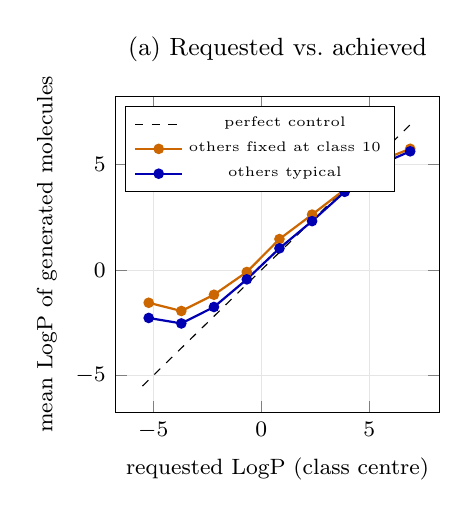
\begin{tikzpicture}
\begin{axis}[width=0.47\textwidth, height=5.6cm, xlabel={requested LogP (class centre)}, ylabel={mean LogP of generated molecules},
  title={\small (a) Requested vs.\ achieved}, grid=major, grid style={black!10}, legend pos=north west, legend style={font=\tiny},
  tick label style={font=\footnotesize}, label style={font=\footnotesize}, title style={yshift=1mm}]
\addplot[black, dashed] coordinates {(-5.5,-5.5) (7,7)};
\addplot[orange!80!black, thick, mark=*, mark size=1.5pt] coordinates {(-5.21,-1.55) (-3.70,-1.94) (-2.19,-1.17) (-0.67,-0.09) (0.84,1.47) (2.35,2.63) (3.86,3.82) (5.38,5.14) (6.89,5.75)};
\addplot[blue!70!black, thick, mark=*, mark size=1.5pt] coordinates {(-5.21,-2.27) (-3.70,-2.53) (-2.19,-1.75) (-0.67,-0.44) (0.84,1.03) (2.35,2.32) (3.86,3.71) (5.38,4.96) (6.89,5.63)};
\legend{perfect control, others fixed at class 10, others typical}
\end{axis}
\end{tikzpicture}\hfill
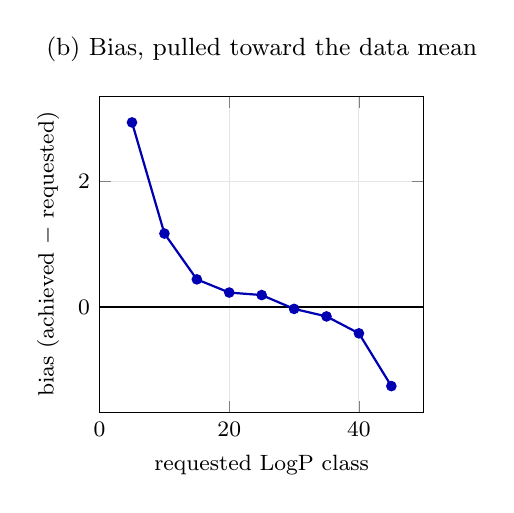
\begin{tikzpicture}
\begin{axis}[width=0.47\textwidth, height=5.6cm, xlabel={requested LogP class}, ylabel={bias (achieved $-$ requested)},
  title={\small (b) Bias, pulled toward the data mean}, grid=major, grid style={black!10}, xmin=0, xmax=50,
  tick label style={font=\footnotesize}, label style={font=\footnotesize}, title style={yshift=1mm}]
\addplot[black, thin] coordinates {(0,0) (50,0)};
\addplot[blue!70!black, thick, mark=*, mark size=1.5pt] coordinates {(5,2.94) (10,1.17) (15,0.44) (20,0.23) (25,0.19) (30,-0.03) (35,-0.15) (40,-0.42) (45,-1.26)};
\end{axis}
\end{tikzpicture}
\caption{The scan of requested LogP classes. (a) The mean LogP that RDKit measures for the generated molecules against the class requested (error bars omitted, see the Std column). The blue curve (typical QED and SAS) follows the diagonal in the dense middle of the range and flattens in both tails. (b) The bias of the blue curve: low requests are answered with too-high LogP, high requests with too-low LogP.}
\label{fig:scan}
\end{figure}

Four observations (all from the table above, and derived in Supplement~\hyperref[sec:S6]{S6}):
\begin{enumerate}[nosep]
  \item \textbf{In the dense middle the mean is honored.} For classes 20 to 35 the mean error is only $0.15$ LogP units, about half a class width. Over classes 15 to 40 the achieved-vs.-requested slope is $0.89$.
  \item \textbf{In the sparse tails the response collapses toward the data.} Class 5 (4 molecules) is requested at $-5.21$ and answered with $-2.27$; class 45 (7 molecules) at $6.89$ and answered with $5.63$. In every class except class 30 (where the bias is negligible) the bias points toward the center of the data (the mean LogP in the data is about $2.5$). The size of the bias correlates strongly with sparsity: $-0.87$ between $|\text{bias}|$ and $\log_{10}$ of the molecules in the class. A plausible reading is that the model, having seen few molecules of a class, smooths across neighboring classes and so pulls extreme requests inward. We have not tested that mechanism.
  \item \textbf{Realistic combinations help.} Averaged over the dense classes 20 to 35, the mean absolute bias is $0.15$ with typical QED and SAS but $0.38$ with both fixed at class 10, and over all nine classes $0.76$ against $1.04$. The ``fixed'' request is an unrealistic combination, and the model pays for it.
  \item \textbf{Validity depends on the request, not simply on the count.} Validity is $92$ to $96\%$ for classes 5 to 35, including the very sparse classes 5 and 10, and drops to $83\%$ and $82\%$ at the high-LogP classes 40 and 45. So it is not just a function of how many molecules a class holds. With the ``fixed'' request it is lower almost everywhere ($79$ to $90\%$).
\end{enumerate}

\subsection*{The spread matters as much as the mean}
Even where the mean is right, the generated LogP values \emph{spread} around the request. The class is $0.30$ units wide, but the standard deviation of the generated molecules is $0.67$ to $1.04$, that is $2.2$ to $3.4$ class widths. If values were scattered uniformly inside a single class the standard deviation would be only $0.30/\sqrt{12}=0.087$. This is a generative model, not a calculator: it controls the \emph{distribution}, not each molecule.

What does that mean for someone who wants a molecule \emph{inside} the requested class? If the generated LogP values are roughly normal (not checked), the fraction of valid molecules landing in the class is about:

\begin{center}
\small
\begin{tabular}{@{}lccccccccc@{}}
\toprule
Class & 5 & 10 & 15 & 20 & 25 & 30 & 35 & 40 & 45\\
\midrule
P(in class) & $0.002$ & $0.06$ & $0.12$ & $0.14$ & $0.15$ & $0.17$ & $0.17$ & $0.14$ & $0.04$\\
Draws per hit, incl.\ validity & $\approx500$ & $18$ & $9.0$ & $7.7$ & $7.2$ & $6.4$ & $6.1$ & $8.5$ & $31$\\
\bottomrule
\end{tabular}
\end{center}

Even in the best classes only about one molecule in six lands in the requested class. Filtering the output by measuring each molecule (\emph{rejection sampling}) therefore costs roughly six to nine draws per hit in the dense range, but $18$ to $31$ in the sparse classes, and about $500$ in class 5, where the model effectively cannot reach the target. The price is also paid in diversity: the survivors are a narrow slice of what the model can produce.

\subsection*{A second property: QED}
The same scan for QED, again with the other properties typical for the requested class, shows a monotone response but a visible upward bias at low requests: reading the tutorial's Figure~14 (approximately), a request for QED $\approx0.2$ returns molecules of mean QED $\approx0.4$, while at the high end (requested $\approx0.87$) the mean is close to the request. QED is bounded by $1$ and its distribution is strongly skewed toward high values (Figure~2 of the tutorial), so low-QED classes are the sparse ones.

\subsection*{The joint picture}
Properties are not independent. In the tutorial's Figure~15, the generated molecules (colored by requested LogP) are plotted in the LogP--QED plane over the density of the training data. The molecules move from left to right as the requested LogP increases. Those for dense requests stay inside the cloud of training molecules, while those for the extreme requests lie at its edge, where realistic combinations are scarce.

\tryit{Primer \S5. Reproduce the bias column, the slopes ($0.75$ over all classes, $0.89$ over classes 15--40), the correlation $-0.87$, the hit rates, and Figure~\ref{fig:scan}. Full tutorial \S7.3--7.6 runs the scans on the model.}

% =============================================================
\section{Step 8: What can you promise?}
% =============================================================
Putting the experiments together, the honest summary of what this model offers:

\begin{center}
\small
\begin{tabular}{@{}p{4.4cm}p{10.6cm}@{}}
\toprule
Use & What the evidence supports\\
\midrule
Generate molecules around a \textbf{typical} property value & Yes. Mean within about $0.15$ LogP units of the request in the dense middle (classes 20--35); validity $93$ to $96\%$.\\
Generate molecules at an \textbf{extreme} value & Only partly. Requests are pulled toward the bulk of the data; the mean can miss by $1$ to $3$ LogP units where classes hold fewer than $\sim40$ molecules.\\
Hit one exact value or class & Not directly. The spread is $2$ to $3$ class widths. Use rejection sampling and expect $6$ to $30$ draws per hit.\\
\textbf{Edit} a known molecule's property & Weakly. About $0.3$ units of change per unit requested (approximate), unless the latent vector is noised or replaced.\\
Request several properties at once & Use realistic combinations. Unrealistic ones raise the error by about a factor of $2.5$ in the dense range and lower validity.\\
\bottomrule
\end{tabular}
\end{center}

Always (i) measure the property independently of the model, (ii) check how many training molecules exist near your request, and (iii) request realistic combinations.

\begin{warnbox}[A valid molecule is not a good molecule]
As in Post~B6: passing RDKit's checks does not make a structure stable, synthesizable or useful. In a conditional model there is a second caution. The model's own labels (and RDKit's recomputation) are \emph{computed} properties, and a molecule that matches a computed LogP is not thereby known to have that measured solubility.
\end{warnbox}

% =============================================================
\section{Run it yourself in Colab}
\label{sec:runit}
% =============================================================
\begin{keybox}[Which notebook?]
\begin{description}[leftmargin=0pt, nosep, labelindent=0pt]
  \item[Primer] \colabbutton{\colaburlprimer}{Open the primer}\ \ \texttt{B6b\_cvae\_primer\_colab.ipynb}. CPU only, a few seconds plus the data download, no model file. It reproduces the data facts, the parameter count, and all of the mathematics of Steps~1--7, analyzes the tutorial's scan results, and ends with a self-check cell. Start here.
  \item[Full tutorial] \colabbutton{\colaburlfull}{Open the full tutorial}\ \ \texttt{TCVAE\_Tutorial.ipynb}. Needs a \textbf{GPU runtime} (a T4 is enough) and the pre-trained model file. It runs the model: latent diagnostics, probes, sampling, the editing test, the scans with $300$ samples per class, and 3D molecule views.
\end{description}
\end{keybox}

\begin{warnbox}[Security note on the model file]
The pre-trained model is distributed as \texttt{CVAE\_transformer\_model.pckl}, a Python \emph{pickle}. A pickle can execute arbitrary code when loaded, so load one only if you received it from a source you trust. The full tutorial also accepts a weights-only file, \texttt{CVAE\_transformer\_state\_dict.pt}, loaded with \texttt{weights\_only=True}, which contains only numbers; it has a cell that exports one from a trusted pickle.
\end{warnbox}

\subsection{Where each step lives}
\begin{center}
\small
\begin{tabular}{@{}llp{6.4cm}@{}}
\toprule
Post & Notebook & What you should see\\
\midrule
Step 1 & Primer \S1; Full \S3 & Tokens $[79,125,147]$; class counts; $22{,}148$ occupied cells\\
Step 2 & Primer \S2 & Parameter table totaling $23{,}046{,}693$; change $+1{,}186{,}724$\\
Step 4a & Primer \S3; Full \S6.2 & Penalty $3.823$ and $3.291$; same penalty for different shapes\\
Step 4b & Primer \S4; Full \S6.2 & Probe $R^2$ and the noise toy model\\
Step 5 & Primer \S6; Full \S6.3 & The metrics table with error bars\\
Step 6 & Primer \S5; Full \S7.2 & Editing slope $\approx0.3$\\
Step 7 & Primer \S5; Full \S7.3--7.6 & Scan table, bias, slopes, hit rates, Figure~\ref{fig:scan}\\
\bottomrule
\end{tabular}
\end{center}

\subsection{The key calculations in one cell}
This script needs only the Python standard library and reproduces the latent-length penalty, the noise toy model, and the hit-rate estimate:

\begin{lstlisting}
import numpy as np
from math import erf, sqrt, exp

d = 1280; s = d * d * 0.0005; w = 4                  # kernel k(x, y) = exp(-|x - y|^2 / s); penalty weight 4

def penalty(L):                                      # simplified penalty for latent vectors of length L
    return w * (1 - (1 + 2 / s) ** (-d / 2) * exp(-L**2 / (s + 2)))

print("prior vs prior :", round(w * (1 - (1 + 4 / s) ** (-d / 2)), 3), "  (measured 3.820)")
print("|z| = 11.8     :", round(penalty(11.8), 3), "  (measured 3.282)")
print("|z| = 0        :", round(penalty(0.0), 3), "  <- the minimum")

v = 0.33**2                                          # variance of an encoder coordinate
for name, r2 in (("LogP", 0.617), ("QED", 0.624), ("SAS", 0.742)):
    snr = r2 / (1 - r2) * v / (v + 1)                # unit noise lowers the signal-to-noise ratio
    print(f"{name}: probe R2 {r2:.3f} -> with unit noise (toy model) {snr / (1 + snr):.3f}")

Phi = lambda x: 0.5 * (1 + erf(x / sqrt(2)))
half = 0.3026 / 2                                    # half-width of a LogP class
for cls, bias, sd, valid in ((30, -0.03, 0.71, 0.933), (10, 1.17, 1.00, 0.917)):
    hit = Phi((half - bias) / sd) - Phi((-half - bias) / sd)
    print(f"LogP class {cls}: P(in class) ~ {hit:.3f}, about {1 / (hit * valid):.1f} draws per molecule in the class")
\end{lstlisting}

Expected output:
\begin{lstlisting}[language={},basicstyle=\ttfamily\small]
prior vs prior : 3.823   (measured 3.820)
|z| = 11.8     : 3.291   (measured 3.282)
|z| = 0        : 3.16   <- the minimum
LogP: probe R2 0.617 -> with unit noise (toy model) 0.137
QED: probe R2 0.624 -> with unit noise (toy model) 0.140
SAS: probe R2 0.742 -> with unit noise (toy model) 0.220
LogP class 30: P(in class) ~ 0.169, about 6.4 draws per molecule in the class
LogP class 10: P(in class) ~ 0.061, about 17.9 draws per molecule in the class
\end{lstlisting}

\subsection{Experiments worth five minutes}
\begin{itemize}[nosep]
  \item \textbf{Find the minimum.} Evaluate \texttt{penalty(L)} for $L$ from $0$ to $40$. Where does it reach the value of two prior samples?
  \item \textbf{Change the weight.} Set \texttt{w = 8}. Which numbers change and which do not? (Hint: only the scale.)
  \item \textbf{A noisier world.} Make the unit noise in the toy model smaller or larger and plot the probe $R^2$ against the noise variance. How much noise leaves the property information almost intact?
  \item \textbf{Tails.} For the scan classes 5 and 45, how many draws would you need for 10 hits?
\end{itemize}

% =============================================================
\section{What to take away}
% =============================================================
\begin{keybox}[Summary]
\begin{itemize}[nosep]
  \item A \textbf{conditional} model describes $p(x\mid c)$. Here the condition is three property classes, turned into tokens and embedded, then concatenated with the latent vector before the decoder.
  \item Equal-width classes leave the \textbf{tails of the property distributions nearly empty} (4 molecules in LogP class 5, 7 in class 45), and the joint (LogP, QED, SAS) cells even more so.
  \item The simplified MMD penalty depends \textbf{only on the length} of each latent vector, so it cannot enforce a match to the prior; the noise added in training is what makes sampling work.
  \item The latent vector of a real molecule \textbf{already carries its properties} ($R^2$ of $0.62$ to $0.74$), which may explain why editing a molecule responds to the condition only weakly (about $0.3\times$) while sampling follows it well in the dense range.
  \item \textbf{Control works as far as the data go}: mean within $\sim0.15$ LogP units in the dense middle, pulled toward the data mean in sparse tails, and always \textbf{spread} over $2$ to $3$ class widths.
  \item Test control with an independent measurement, request \textbf{realistic} combinations, and filter by measurement if you need an exact value.
\end{itemize}
\end{keybox}

\textbf{Next in the series (B7):} predicting dynamics with dynamic mode decomposition.

\vspace{0.5em}
{\footnotesize\textbf{Credits and license.} The tutorial notebook, \textit{Conditional VAE Transformer (TCVAE): generating molecules with desired properties}, is by Prof.\ Victor S.\ Batista (CHEM~584, Yale), version~1.0, November 2026; an earlier version of the assignment was designed by Dr.\ Haote Li. Text is CC~BY~4.0 and code is MIT, per the notebook. The ZINC subset is distributed with the \texttt{chemical\_vae} repository of the Aspuru-Guzik group.}

\clearpage
% =============================================================
\section*{Supplementary Reading: The Math}
\addcontentsline{toc}{section}{Supplementary Reading: The Math}
% =============================================================
\textit{Prerequisites: Post B6 (its supplement S4 on MMD), expectations of Gaussians, and the basic statistics of Toolbox T3.}

\phantomsection\label{sec:S1}
\subsection*{S1. Conditional generative models}
A generative model of $x$ given $c$ is trained to maximize $\ln p_\theta(x\mid c)$. The \textbf{conditional VAE} (Sohn et al., 2015) introduces a latent variable $z$ and an encoder $q_\phi(z\mid x,c)$, and maximizes the conditional evidence lower bound
\[
  \ln p_\theta(x\mid c)\ \ge\ \E_{q_\phi(z\mid x,c)}\!\big[\ln p_\theta(x\mid z,c)\big]-\mathrm{KL}\big(q_\phi(z\mid x,c)\,\big\|\,p(z)\big),
\]
with a prior $p(z)=N(0,I)$ that does \emph{not} depend on $c$. To generate, draw $z\sim p(z)$ and decode $p_\theta(x\mid z,c)$ for the $c$ you choose.

\paragraph{What this model does instead.} The encoder is deterministic and the KL term is replaced by an MMD-type penalty on the \emph{marginal} distribution of $z$ (all molecules, all conditions mixed). The decoder is a Transformer with the memory built from $[z\,|\,c]$, as in Figure~\ref{fig:arch}.

\paragraph{The independence assumption and its leakage.} Sampling $z$ from a prior that does not depend on $c$ presumes that the latent variable is (approximately) independent of the condition: the encoder should store in $z$ only what $c$ does \emph{not} already explain. Nothing in this training objective enforces that. The penalty acts on the marginal of $z$, and the encoder sees $c$ in its input, so $z$ may carry information about $c$. The probe of Step~4b shows that it does: held-out $R^2$ of $0.62$ to $0.74$. Then the distribution of $z$ given $c$ differs from the marginal prior, and the pair $(z,c)$ that we feed at generation time (random $z$, chosen $c$) can be inconsistent with the pairs seen in training. Approaches that explicitly remove attribute information from $z$ include adversarial training against a classifier that predicts the attribute from the latent code (the Fader networks of Lample et al., 2017).

\phantomsection\label{sec:S2}
\subsection*{S2. Discretization of a continuous property}
For a property with minimum $a$ and maximum $b$ and $K=50$ classes, the class width is $\Delta=(b-a)/K$ and class $k\in\{0,\dots,K-1\}$ covers $[a+k\Delta,\ a+(k+1)\Delta)$. The notebook computes a molecule's class as the number of class lower edges below its value, clipped to at least $1$ (so the minimum falls in class 0), minus one:
\[
  k=\operatorname{clip}\big(\#\{j:\ e_j<x\},\,1,\,K\big)-1,\qquad e_j=a+j\Delta .
\]
\paragraph{Resolution.} If the property were uniformly spread inside the class, the discretization error would have variance $\Delta^2/12$, so a standard deviation $\Delta/\sqrt{12}$: $0.087$ LogP units here. This is the \emph{best case} for the precision of a request; the achieved spread (Step~7) is $8$ to $12$ times larger.

\paragraph{Resolution against sparsity.} More classes give finer requests, but fewer molecules per class. If a property has density $f$, class $k$ is expected to hold about $N f(x_k)\Delta$ molecules, and a count of $n$ has relative statistical uncertainty $\approx1/\sqrt n$. With $K=50$ the middle LogP class holds $20{,}044$ molecules (relative uncertainty under $1\%$) while class 5 holds $4$ ($50\%$). With three properties the problem compounds: $K^3=125{,}000$ cells for $249{,}455$ molecules, of which $22{,}148$ are occupied.

\phantomsection\label{sec:S3}
\subsection*{S3. Counting the parameters of the conditional model}
Use the building blocks of Post~B6's S3: a linear layer $m\to n$ has $mn+n$ parameters, a layer normalization $2n$, an embedding table $rH$, an attention block $4(H^2+H)=66{,}048$, a feed-forward block $65{,}920$, an encoder layer $132{,}480$ and a decoder layer $198{,}784$ (with $H=128$, feed-forward width $256$). The conditional model uses $190$ input tokens, $37$ output tokens, $200$ positions, a row length of $115$ and an inverse layer with $1664$ inputs:
\begin{align*}
  \text{encoder}&=190\cdot128+200\cdot128+6\cdot132{,}480=844{,}800,\\
  \text{decoder}&=37\cdot128+200\cdot128+6\cdot198{,}784+(128\cdot37+37)=1{,}227{,}813,\\
  \text{latent layer}&=115\cdot128\cdot1280+1280=18{,}842{,}880,\\
  \text{inverse layer}&=1664\cdot1280+1280=2{,}131{,}200,\\
  \text{total}&=844{,}800+1{,}227{,}813+18{,}842{,}880+2{,}131{,}200=23{,}046{,}693 .
\end{align*}
Relative to the unconditional model ($21{,}859{,}969$) the changes are: encoder embeddings $+29{,}824$ (the larger token and position tables), decoder position table $+10{,}240$, latent layer $+655{,}360$ ($512$ extra inputs $\times\,1280$), inverse layer $+491{,}520$ ($384$ extra inputs $\times\,1280$), and the two residual blocks $-220$. The sum is $+1{,}186{,}724$.

\phantomsection\label{sec:S4}
\subsection*{S4. The cross-term penalty sees only the length of $z$}
With the Gaussian kernel $k(\bm x,\bm y)=\exp(-\lVert\bm x-\bm y\rVert^2/s)$ and a prior sample $\bm y\sim N(0,I_d)$, fix a latent vector $\bm z$. The squared distance $\lVert\bm z-\bm y\rVert^2$ follows a \emph{noncentral} $\chi^2_d$ distribution with noncentrality $\lambda=\lVert\bm z\rVert^2$, whose moment generating function is
\[
  \E\,e^{-tX}=(1+2t)^{-d/2}\exp\!\Big(-\frac{t\lambda}{1+2t}\Big)\qquad(X\sim\chi'^2_d(\lambda),\ t>-\tfrac12).
\]
With $t=1/s$:
\begin{equation}
  \E_{\bm y}\,k(\bm z,\bm y)=\Big(1+\frac2s\Big)^{-d/2}\exp\!\Big(-\frac{\lVert\bm z\rVert^2}{s+2}\Big).
\end{equation}
The direction of $\bm z$ has disappeared: the average kernel depends on $\bm z$ only through $\lVert\bm z\rVert$. The penalty for a batch is therefore
\[
  \text{penalty}=w\Big[1-\Big(1+\tfrac2s\Big)^{-d/2}\cdot\tfrac1n\sum_{i=1}^n e^{-\lVert\bm z_i\rVert^2/(s+2)}\Big],
\]
which is Eq.~\eqref{eq:lenpen}. Each term $e^{-L^2/(s+2)}$ is strictly decreasing in $L=\lVert\bm z_i\rVert$, so the penalty is strictly \emph{increasing} in every length and minimal when all vectors are at the origin, where it equals $w[1-(1+2/s)^{-d/2}]=3.160$ for $w=4$. Two consequences: the penalty \textbf{cannot detect that the vectors are squeezed into a few directions} (the primer builds two sets of equal-length vectors, one with $88\%$ of its variance in $20$ of $1280$ coordinates, and both give $3.291$), and it \textbf{rewards shrinkage}. The cross-entropy term pushes back, since the decoder needs $\bm z$ to carry information, and the encoder settles where the two forces balance; we showed the direction of the pull, not the location of the equilibrium.

\paragraph{Two prior samples.} If both vectors come from $N(0,I_d)$ then $\lVert\bm y'\rVert^2\sim\chi^2_d$ and $\E\,e^{-\lVert\bm y'\rVert^2/(s+2)}=(1+\tfrac{2}{s+2})^{-d/2}$. Since $(1+\tfrac2s)(1+\tfrac2{s+2})=\tfrac{s+2}{s}\cdot\tfrac{s+4}{s+2}=1+\tfrac4s$, the product is $(1+4/s)^{-d/2}$ and the penalty is $w[1-(1+4/s)^{-d/2}]=3.823$ for $w=4$ (measured $3.820$).

\paragraph{The full MMD.} The full estimator of Post~B6 adds the terms $\E\,k(\bm z,\bm z')$ and $\E\,k(\bm y,\bm y')$. The first one compares the vectors with \emph{each other} and does depend on their directions, which is what lets the full estimator tell an isotropic cloud from a squeezed one. The tutorial's code leaves the full version as a commented-out line.

\phantomsection\label{sec:S5}
\subsection*{S5. A toy model of the probe and the noise}
Let $y$ be a standardized property ($\E y=0$, $\Var y=1$). Model the latent vector as $\bm x=\bm a\,y+\bm n$ with a fixed direction $\bm a\in\R^d$ and other variation $\bm n\sim N(0,v I)$ independent of $y$, where $v$ is the per-coordinate variance of the other variation. Then $\operatorname{Cov}(\bm x)=\bm a\bm a^{\T}+vI$ and $\operatorname{Cov}(y,\bm x)=\bm a^{\T}$, so the best linear estimate of $y$ is $\hat y=\bm a^{\T}\bm x/(\lVert\bm a\rVert^2+v)$ (by the Sherman--Morrison formula, $(\bm a\bm a^{\T}+vI)^{-1}\bm a=\bm a/(\lVert\bm a\rVert^2+v)$), and its coefficient of determination is
\[
  R^2=\bm a^{\T}(\bm a\bm a^{\T}+vI)^{-1}\bm a=\frac{\lVert\bm a\rVert^2}{\lVert\bm a\rVert^2+v}=\frac{\mathrm{SNR}}{1+\mathrm{SNR}},\qquad \mathrm{SNR}=\frac{\lVert\bm a\rVert^2}{v}.
\]
Adding independent noise $\bm\varepsilon\sim N(0,I)$ raises the noise variance from $v$ to $v+1$ per coordinate, so
\[
  \mathrm{SNR}'=\frac{\lVert\bm a\rVert^2}{v+1}=\mathrm{SNR}\cdot\frac{v}{v+1}.
\]
Inverting the first formula for the measured probe values gives $\mathrm{SNR}=R^2/(1-R^2)=1.61,\ 1.66,\ 2.88$ for LogP, QED and SAS. With $v=0.33^2=0.109$, the factor is $v/(v+1)=0.098$, so $\mathrm{SNR}'=0.158,\ 0.163,\ 0.283$ and
\begin{center}
\small
\begin{tabular}{@{}lccc@{}}
\toprule
 & LogP & QED & SAS\\
\midrule
$R^2$ from the clean $\bm z$ (measured) & $0.617$ & $0.624$ & $0.742$\\
$R^2$ with unit noise (toy model) & $0.137$ & $0.140$ & $0.220$\\
\bottomrule
\end{tabular}
\end{center}
\paragraph{Assumptions.} The model assumes a single signal direction, isotropic other variation of variance $\sigma_z^2$ per coordinate, and an optimal linear readout. The real latent vectors are far from isotropic (the first principal component carries a variance of about $3.7$ against an average coordinate variance of $0.11$, read from the tutorial's Figure~6b). The numbers are therefore an order-of-magnitude illustration of a mechanism, not a measurement of the decoder. Its testable prediction: if the decoder learned to rely on $\bm c$ because the noise hides the property in $\bm z$, then (i) adding noise to $\bm z$ in the editing test should increase the response to the condition, and (ii) a decoder trained without noise should rely on $\bm z$ more.

\phantomsection\label{sec:S6}
\subsection*{S6. Measuring control: bias, slope, spread and hit rate}
For a request of class center $r$, let $\bar x$ be the mean of the measured property of $n_v$ valid generated molecules and $\sigma$ their standard deviation. Then
\[
  \text{bias}=\bar x-r,\qquad \mathrm{SE}(\bar x)=\frac{\sigma}{\sqrt{n_v}} .
\]
With $n=300$ samples per class and validity $\approx0.9$, $\mathrm{SE}\approx0.04$ to $0.06$. Judged against these, the biases are statistically significant in almost every class (for example $+0.19$ at class 25 is about $4\,\mathrm{SE}$; only class 30, $-0.03$, is consistent with zero), but \emph{practically} small in the dense classes: under $0.25$ LogP units, below one class width. The error bars in the tutorial's plots are the spread $\sigma$, not $\mathrm{SE}$.

\paragraph{Slope.} A least-squares fit of the achieved mean against the requested value over the nine classes gives slope $0.75$ (typical) and $0.70$ (fixed). Over classes 15 to 40 the slopes are $0.89$ and $0.84$. The mean absolute bias is $0.76$ against $1.04$ over all nine classes, and $0.15$ against $0.38$ over classes 20 to 35.

\paragraph{Sparsity.} The correlation between $|\text{bias}|$ and $\log_{10}$(molecules in class) is $-0.87$ for the typical requests and $-0.82$ for the fixed requests. The bias has the sign of ``toward the data mean'' in every class except class 30, where it is negligible (positive below the mean LogP of about $2.5$, negative above). A plausible interpretation is smoothing across neighboring classes in the learned conditional distribution; the experiment does not distinguish this from other explanations.

\paragraph{Hit rate.} If the generated values are approximately $N(r+b,\sigma^2)$ with bias $b$ and the class has half-width $h=\Delta/2=0.151$, the probability that a generated value lies in the class is
\[
  P_{\rm hit}=\Phi\!\Big(\frac{h-b}{\sigma}\Big)-\Phi\!\Big(\frac{-h-b}{\sigma}\Big),
\]
and the expected number of draws per molecule inside the class, including the chance that a draw is invalid with validity $q$, is $1/(P_{\rm hit}\,q)$. For class 30 ($b=-0.03$, $\sigma=0.71$, $q=0.933$): $P_{\rm hit}=\Phi(0.254)-\Phi(-0.169)=0.600-0.433=0.169$, so $6.4$ draws. For class 10 ($b=1.17$, $\sigma=1.00$, $q=0.917$): $P_{\rm hit}=0.061$, so $17.9$ draws. These use the normal approximation, which we did not check, and ignore any correlation between validity and property value, so they are estimates of the order of magnitude.

\phantomsection\label{sec:S7}
\subsection*{S7. Reading the sampling table}
As in Post~B6's S7, with $n=5000$: $n_v=4882$, $n_d=4861$ distinct among the valid, $n_n=4857$ novel, so validity $0.9764$, uniqueness $0.9957$, novelty $0.9992$, and yield $n_n/n=0.9714$. The interval half-widths $1.96\sqrt{\hat p(1-\hat p)/n}$ are $0.42$ for validity and $1.38$ for the reconstruction accuracy $0.532$.

\paragraph{A comparison that needs care.} The unconditional model's yield is $76.06\%$ and the conditional model's is $97.14\%$. But the two models differ in architecture, training and penalty weight, and the conditional test samples at one dense condition. In the scan, validity for typical requests ranges from $81.7\%$ to $95.7\%$ and for fixed requests from $78.7\%$ to $90.0\%$. A fair comparison would use the same data, the same training budget and the same set of requests.

\phantomsection\label{sec:S8}
\subsection*{S8. Beyond this model}
\begin{itemize}[nosep]
  \item \textbf{Condition dropout.} Randomly hide the condition tokens during training so that the same network also learns the unconditional distribution (Exercise~7). This is the idea behind classifier-free guidance (Ho and Salimans, 2022): at generation time one can then interpolate or extrapolate between the conditional and unconditional predictions to strengthen the control.
  \item \textbf{Removing property information from $\bm z$.} Adversarial or mutual-information penalties that make $\bm z$ uninformative about $\bm c$ address the leakage of Supplement~S1 directly (Lample et al., 2017).
  \item \textbf{Continuous conditions.} Discretizing into classes is simple but sparse (S2). Feeding the property as a number, with an embedding network, avoids the empty classes but needs care to keep requests in the supported range.
  \item \textbf{Fixing the penalty.} Replacing the cross-term penalty with the full MMD estimator (Exercise~6) removes the pull toward the origin (S4); whether it improves the control is an experiment worth running.
\end{itemize}

\subsection*{Check yourself}
\begin{enumerate}
  \item \textbf{Tokens.} A molecule has LogP $=2.5$, QED $=0.75$, SAS $=2.2$. Compute its three classes and tokens by hand with the ranges and widths of Step~1, then check with the primer (Exercise~1).
  \item \textbf{Parameters.} How many parameters would the encoder embedding table gain if there were $100$ classes per property instead of $50$? Which other layers would change?
  \item \textbf{The penalty.} Compute Eq.~\eqref{eq:lenpen} for $\lVert\bm z\rVert=5,\ 20,\ 35.8$. Which length does the penalty prefer? Why does the answer not depend on the weight $w$?
  \item \textbf{Noise.} In the toy model of S5, how large must the noise variance be to push the QED probe $R^2$ below $0.05$?
  \item \textbf{A testable prediction (full tutorial).} In the editing test of Step~6, add $N(0,I)$ noise to each latent vector before decoding. If the hypothesis is right, what should happen to the slope? What would it mean if nothing changed? Also replace $\bm z$ by a random draw for each molecule (Exercise~5 of the tutorial) and predict the slope using the scan.
  \item \textbf{Hit rate.} How many draws are needed on average to obtain $100$ molecules inside LogP class $35$? Inside class $10$? Why is the class-10 estimate optimistic?
  \item \textbf{Condition dropout.} Sketch how you would change the training loop to hide the condition tokens $20\%$ of the time. What would you use for the missing condition? What can you do at generation time that you could not do before?
  \item \textbf{The full MMD.} Replace the simplified penalty by the full estimator and predict how the encoded-vector length and the editing slope would change.
\end{enumerate}

\subsection*{References}
{\small\sloppy
\begin{itemize}[nosep, leftmargin=1.2em]
  \item K.~Sohn, H.~Lee, X.~Yan, \textit{Learning structured output representation using deep conditional generative models}, NeurIPS 28 (2015).
  \item J.~Lim, S.~Ryu, J.~W.~Kim, W.~Y.~Kim, \textit{Molecular generative model based on conditional variational autoencoder for de novo molecular design}, J.\ Cheminform.\ \textbf{10}, 31 (2018).
  \item S.~Kang, K.~Cho, \textit{Conditional molecular design with deep generative models}, J.\ Chem.\ Inf.\ Model.\ \textbf{59}, 43--52 (2019).
  \item G.~Lample et al., \textit{Fader networks: manipulating images by sliding attributes}, NeurIPS 30 (2017).
  \item J.~Ho, T.~Salimans, \textit{Classifier-free diffusion guidance} (2022), arXiv:2207.12598.
  \item A.~Vaswani et al., \textit{Attention is all you need}, NeurIPS 30 (2017), arXiv:1706.03762.
  \item D.~P.~Kingma, M.~Welling, \textit{Auto-encoding variational Bayes}, ICLR (2014), arXiv:1312.6114.
  \item S.~Zhao, J.~Song, S.~Ermon, \textit{InfoVAE: Information maximizing variational autoencoders} (2017), arXiv:1706.02262.
  \item A.~Gretton et al., \textit{A kernel two-sample test}, J.\ Mach.\ Learn.\ Res.\ \textbf{13}, 723--773 (2012).
  \item R.~G\'omez-Bombarelli et al., \textit{Automatic chemical design using a data-driven continuous representation of molecules}, ACS Cent.\ Sci.\ \textbf{4}, 268--276 (2018).
  \item G.~R.~Bickerton et al., \textit{Quantifying the chemical beauty of drugs}, Nat.\ Chem.\ \textbf{4}, 90--98 (2012). (QED.)
  \item S.~A.~Wildman, G.~M.~Crippen, \textit{Prediction of physicochemical parameters by atomic contributions}, J.\ Chem.\ Inf.\ Comput.\ Sci.\ \textbf{39}, 868--873 (1999). (Crippen LogP.)
  \item P.~Ertl, A.~Schuffenhauer, \textit{Estimation of synthetic accessibility score of drug-like molecules}, J.\ Cheminform.\ \textbf{1}, 8 (2009). (SAS.)
  \item D.~Weininger, \textit{SMILES, a chemical language and information system}, J.\ Chem.\ Inf.\ Comput.\ Sci.\ \textbf{28}, 31--36 (1988).
  \item T.~Sterling, J.~J.~Irwin, \textit{ZINC 15 --- ligand discovery for everyone}, J.\ Chem.\ Inf.\ Model.\ \textbf{55}, 2324--2337 (2015).
  \item D.~Polykovskiy et al., \textit{Molecular Sets (MOSES)}, Front.\ Pharmacol.\ \textbf{11}, 565644 (2020).
  \item N.~Brown et al., \textit{GuacaMol: benchmarking models for de novo molecular design}, J.\ Chem.\ Inf.\ Model.\ \textbf{59}, 1096--1108 (2019).
\end{itemize}}

\end{document}
